\subsubsection{Theo kiểu cũ - ở LearnOpenGL}
\begin{enumerate}
    \item Tại thư mục src, tạo file main.cpp.
    \item Tại dòng đầu của file main.cpp, gọi thư viện glad.h (glad trước glwr
     thì mới gọi ra được con trỏ các hàm của glwr), rồi gọi thư viện glwr.h.
     %hiển thị code, nền đen

    \begin{lstlisting}[language=C++]
        #include <glad/glad.h>
        #include <GLFW/glfw3.h>
    \end{lstlisting}

    \item \textbf{glfwInit()}:

    Việc sử dụng ${\#include <GLFW/glfw3.h>}$ trong mã nguồn của bạn là để
     bao gồm các khai báo và định nghĩa liên quan đến GLFW. Tuy nhiên,
      việc đưa mã nguồn của thư viện vào mã của bạn chỉ
     giúp bạn truy cập các khai báo và hàm từ GLFW mà bạn có thể gọi 
     trong mã của mình. Nó không thực sự khởi tạo hoặc quản lý bất kỳ
      thành phần cụ thể nào của GLFW cho bạn.

      glfwInit() là một hàm cụ thể của GLFW được sử dụng để khởi tạo thư 
      viện GLFW và chuẩn bị môi trường đồ họa. Khi bạn gọi glfwInit(), nó 
      thực sự thực hiện công việc khởi tạo thư viện và cài đặt các
       tài nguyên cần thiết cho việc làm việc với đồ họa.  

    \item \textbf{glfwWindowHint()}:
 
    Hàm glfwWindowHint trong thư viện GLFW được sử dụng để đặt các 
    cài đặt cho cửa sổ đồ họa mà bạn sẽ tạo sau đó bằng hàm glfwCreateWindow.
     Dưới đây là một số cài đặt phổ biến mà bạn có thể sử dụng với glfwWindowHint:
    
\begin{itemize}
    \item \texttt{glfwWindowHint(GLFW\_CONTEXT\_VERSION\_MAJOR, majorVersion)}
      và \\
      \texttt{glfwWindowHint(GLFW\_CONTEXT\_VERSION\_MINOR, minorVersion)}:
      
      Đặt phiên bản của OpenGL bạn muốn sử dụng. Ví dụ, để đặt phiên bản 
      OpenGL 4.5, bạn có thể sử dụng 
     \begin{lstlisting}[language=C++]
        glfwWindowHint(GLFW_CONTEXT_VERSION_MAJOR, 4);
        glfwWindowHint(GLFW_CONTEXT_VERSION_MINOR, 5);
     \end{lstlisting}
     \item \texttt{glfwWindowHint(GLFW\_OPENGL\_PROFILE,
      GLFW\_OPENGL\_CORE\_PROFILE)}:
      Đặt hồ sơ OpenGL bạn muốn sử dụng. Hồ sơ \texttt{ GLFW\_OPENGL\_CORE\_PROFILE 
      }sử dụng phiên bản core của OpenGL, 
      trong khi \texttt{GLFW\_OPENGL\_COMPAT\_PROFILE} sử dụng phiên bản tương thích
       ngược.
      %code 
        \begin{lstlisting}[language=C++]
            glfwWindowHint(GLFW_OPENGL_PROFILE, GLFW_OPENGL_CORE_PROFILE);
        \end{lstlisting}
    \end{itemize}

   \item \textbf {glfwCreateWindow()}:
   %code GLFWwindow* window = glfwCreateWindow(800, 600, "LearnOpenGL", NULL, NULL);
   \begin{lstlisting}[language=C++]
    GLFWwindow* window = glfwCreateWindow(800, 600, "LearnOpenGL", NULL, NULL);
   \end{lstlisting}
   Hàm glfwCreateWindow yêu cầu hai đối số đầu tiên lần lượt 
   là chiều rộng và chiều cao của cửa sổ. Đối số thứ ba 
   cho phép bạn đặt tên cho cửa sổ; hiện tại, bạn gọi nó là 
   "LearnOpenGL" nhưng bạn có thể đặt tên tùy ý. Bạn có thể bỏ 
   qua hai đối số cuối cùng. Hàm trả về một đối tượng GLFWwindow mà
    sau này bạn sẽ cần cho các hoạt động GLFW khác. Sau đó, bạn chỉ 
    định cho GLFW làm cho ngữ cảnh của cửa sổ của 
   bạn trở thành ngữ cảnh chính trên luồng hiện tại.
   \item Giữ cửa sổ ko bị đóng lại:
    %code
    \begin{lstlisting}[language=C++]
        while(!glfwWindowShouldClose(window))
        {
            glfwSwapBuffers(window);
            glfwPollEvents();    
        }
    \end{lstlisting}
      \begin{itemize}
        \item while (!glfwWindowShouldClose(window)): Đây là một
         vòng lặp chạy liên tục cho đến khi biểu thức
          glfwWindowShouldClose(window) trả về giá trị true.
           Hàm này kiểm tra xem GLFW đã được hướng dẫn để đóng cửa sổ hay 
           chưa. Nếu cửa sổ được đóng, biểu thức này trả về true và vòng 
        lặp dừng chạy, sau đó bạn có thể đóng ứng dụng.
        \item glfwSwapBuffers(window): Hàm này thực hiện việc hoán đổi
         (swap) hai bộ đệm màu. GLFW sử dụng hai bộ đệm màu để hiển 
         thị hình ảnh trên cửa sổ. Một bộ đệm được vẽ và lắng nghe dữ
          liệu đồ họa mới (color buffer), trong khi bộ đệm còn lại 
          hiển thị nội dung đã vẽ. Khi bạn gọi glfwSwapBuffers(window),
           nó sẽ chuyển đổi giữa hai bộ đệm, làm cho nội dung đã vẽ 
           xuất hiện trên cửa sổ.
        \item
        glfwPollEvents(): Hàm này kiểm tra xem có sự kiện nào được 
        kích hoạt (như sự kiện nhập từ bàn phím, chuyển động chuột, 
        vv.), cập nhật trạng thái của cửa sổ và gọi các hàm tương ứng 
        (các hàm được đăng ký thông qua các phương thức gọi lại callback).
         Nó giúp bạn xử lý sự kiện và tương tác người dùng trong ứng dụng
          của bạn.
        \item Một số dòng code khác: ko có xài thì cũng vẫn hiện cửa sổ lên.
        \begin{itemize}
            \item \texttt{glViewport(0, 0, 800, 600)}: Đặt kích thước
            \item   
            \texttt{glClearColor(0.2f, 0.3f, 0.3f, 1.0f)}: Đặt màu nền
            \item \texttt{glClear(GL\_COLOR\_BUFFER\_BIT)}: Xóa màu nền
            \item \texttt{glfwTerminate()}: Đóng GLFW
            \item \texttt{glfwSetFramebufferSizeCallback(window,
             framebuffer\_size\_callback)}: Đăng kí hàm callback 
                để khi thay đổi kích thước cửa sổ thì cửa sổ vẫn hiện lên
        \end{itemize}
        \item Tạo 2 cửa sổ: 
        %code
        \begin{lstlisting}[language=C++]
    GLFWwindow* window1 = glfwCreateWindow(width1, height1, 
    "Cua so 1", NULL, NULL);
    if (window1 == NULL) {
        glfwTerminate();
        return -1;
    }

    GLFWwindow* window2 = glfwCreateWindow(width2, height2, 
    "Cua so 2", NULL, NULL);
    if (window2 == NULL) {
        glfwTerminate();
        return -1;
    }
    glfwMakeContextCurrent(window1);
    glfwMakeContextCurrent(window2);

    \end{lstlisting}
    %chèn ảnh
    \begin{figure}[H]
        \centering
        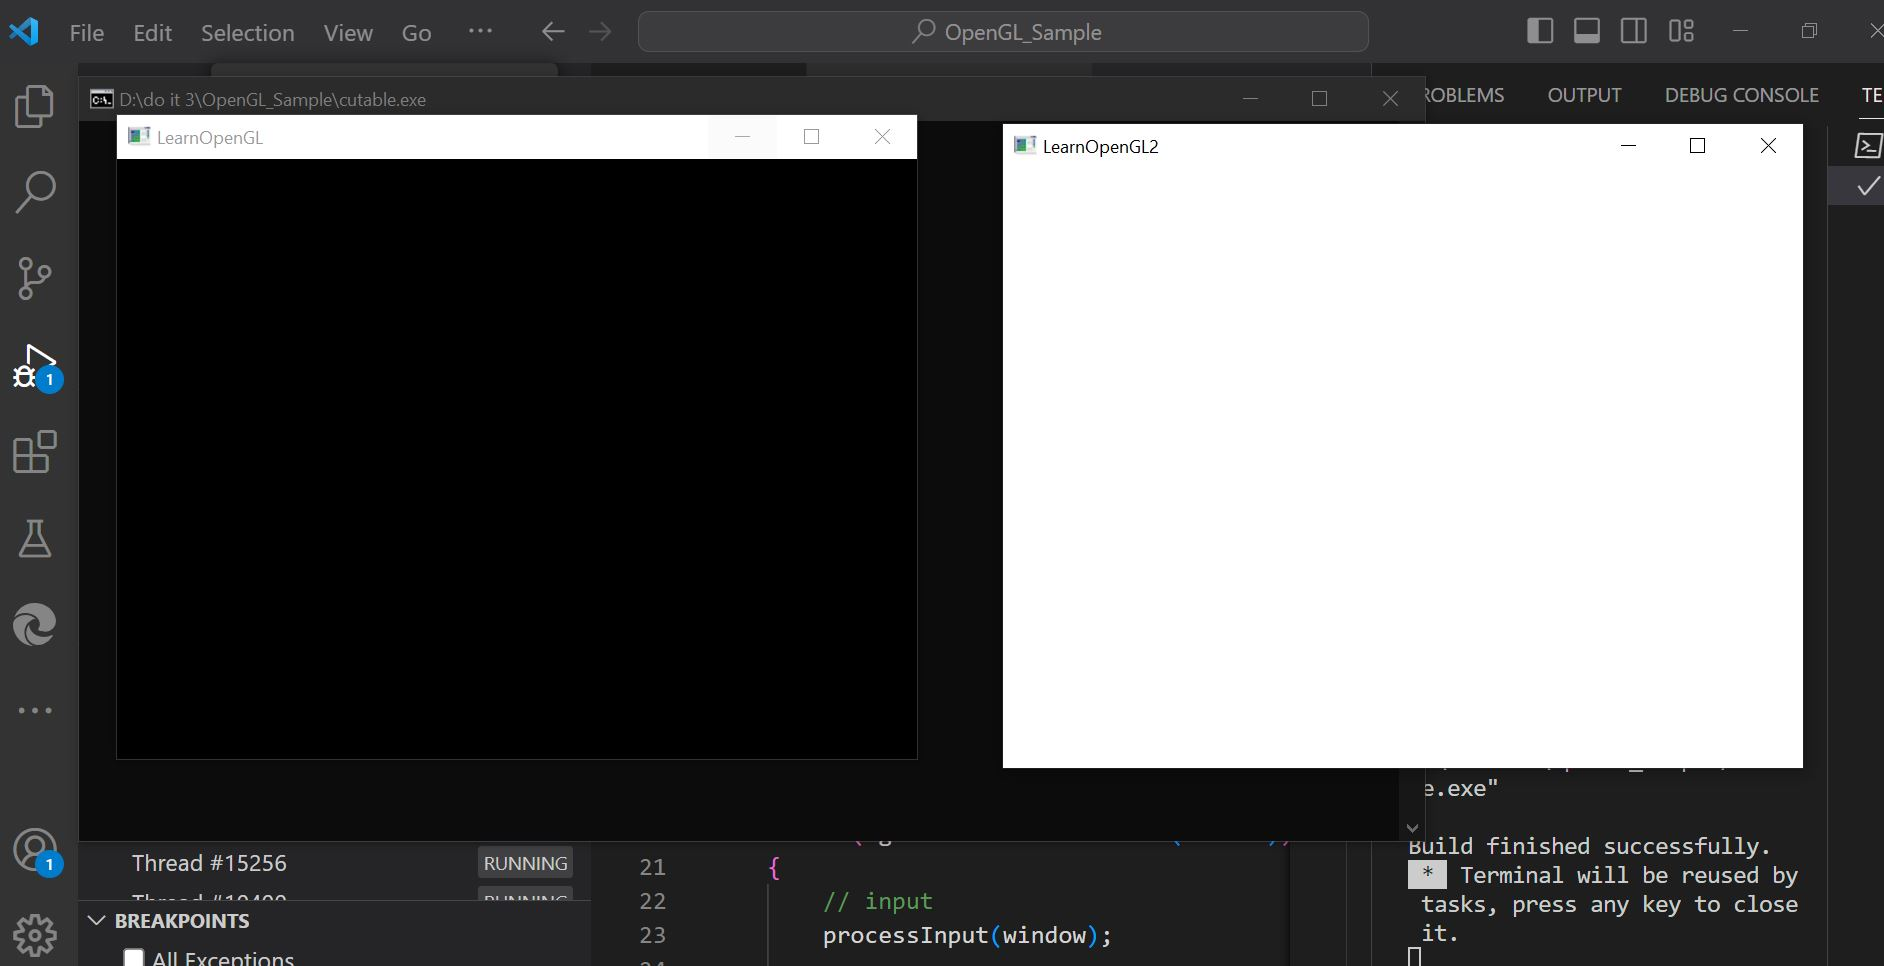
\includegraphics[scale=0.5]{2_windows.JPG}
    \end{figure}
        \item Dòng code xử lí lỗi:
        \begin{itemize}
            \item Lỗi ko tạo được cửa sổ %code 
            \begin{lstlisting}[language=C++]
                if (window == NULL)
                {
                    std::cout << "Failed to create GLFW window" << std::endl;
                    glfwTerminate();
                    return -1;
                }
            \end{lstlisting}
            \item Lỗi ko tạo được ngữ cảnh %code
            \begin{lstlisting}[language=C++]
    glfwMakeContextCurrent(window);
    if (!gladLoadGLLoader((GLADloadproc)glfwGetProcAddress))
    {
        std::cout << "Failed to initialize GLAD" << std::endl;
        return -1;
    }
    \end{lstlisting}
            
\end{itemize}
        
        \end{itemize}
        
        
\end{enumerate}

\subsubsection{Theo kiểu mới - refacted code}

Tạo 1 file tên là \texttt{standard\_includes.cpp} trong thư mục include.
File này sẽ chứa các hàm init\_glfw chứa các hàm con để tạo cửa sổ, tạo ngữ cảnh, tạo vòng lặp 
để giữ cửa sổ ko bị đóng lại, xử lí lỗi, đóng GLFW, ..

Sau đó trong hàm main ta gọi hàm init\_glfw ra và tập trung vào
 việc vẽ hình.